
\documentclass[12pt,a4paper,oneside]{book}
\usepackage[utf8]{inputenc}
\usepackage{amsmath}
\usepackage{amsfonts}
\usepackage{amssymb}
\usepackage[spanish]{babel}
\usepackage[graphicx]{realboxes}
\usepackage{wrapfig}
\usepackage{fancyhdr}
\usepackage[hidelinks]{hyperref}
\usepackage{datatool}
% \usepackage[acronym]{glossaries}
\usepackage{glossaries}
\usepackage{makeidx}
\usepackage{multirow}
\usepackage{multicol}
\usepackage{colortbl}
\usepackage{cite}
\usepackage{IEEEtrantools}
% \usepackage{ieeetrantools}
\usepackage{float}
\makeindex
\pagestyle{fancy}

\makeglossaries % este comando debe estar en el preámbulo

\begin{document}
% \renewcommand{\glossaryname}{Glosario}

\renewcommand\listtablename{\'Indice de Tablas}
%\listtablename

\renewcommand{\tablename}{Tabla}
\renewcommand{\acronymname}{Acr\'onimos y s\'imbolos}
\renewcommand{\bibname}{Referencias bibliogr\'aficas}
%\glsaddall
\frontmatter
\vspace*{-3cm}
\begin{figure}[h]
\leavevmode
\begin{minipage}{\textwidth}
\begin{center}
%\includegraphics[scale=0.5]{./logofpune}
\end{center}
\end{minipage}
\end{figure}

\thispagestyle{empty}

{\bf
\begin{center}
\large
\vspace*{-1 cm}\Large \textsc{Universidad Nacional del Este.} \\
\Large \textsc{Facultad Politécnica.} \\
\vspace*{0.5 cm}\hrule
\end{center}
}

\vspace*{-0.5 cm}
\begin{figure}[htb]
\begin{center}

\includegraphics[scale = .6]{./portada_y_ficha_catalografica/logo.png}

\end{center}
\end{figure}


\vspace{3 cm}
{
\noindent
\begin{center}
\huge \bf $<$Título del Trabajo Final de Grado$>$.
\end{center}
}


\vspace{6 cm}

\begin{center}
{\textbf{\Large $<$Nombre del graduando$>$.}\\[5mm]
\vspace{1 cm}
\textbf{Año \the\year.}}
\end{center}

\bstctlcite{IEEEexample:BSTcontrol} % cambia "and" por "y" en bibliografía

\vspace*{-3cm}
\begin{figure}[h]
\leavevmode
\begin{minipage}{\textwidth}
\begin{center}
%\includegraphics[scale=0.5]{./logofpune}
\end{center}
\end{minipage}
\end{figure}

\thispagestyle{empty}

{\bf
\begin{center}
\large
\vspace*{-1 cm}\Large \textsc{Universidad Nacional del Este.} \\
\Large \textsc{Facultad Politécnica.} \\
\vspace*{0.5 cm}\hrule
\vspace*{0.5 cm}\Large Carrera $<$Nombre de la Carrera$>$.\\
\vspace*{0 cm}\Large Cátedra $<$Nombre de la Cátedra$>$.\\
\end{center}
}

\vspace{3.5 cm}
{
\noindent
\begin{center}
\huge \bf $<$Título del Trabajo Final de Grado$>$.
\end{center}
}


\vspace{0.5 cm}
{ 

Por: \textbf{\Large $<$Nombre del graduando$>$.}

\vspace*{.5 cm}
Profesor Orientador: \textbf{\large $<$Nombre del Profesor Orientador$>$.}
}%\\[6mm]
\vspace*{0.5 cm}\\
Trabajo final de grado presentado a la Facultad Politécnica de la Universidad Nacional del Este como parte de los requisitos para optar al título $<$denominación del título de grado$>$.

\vspace{4.0cm}
\begin{center}
{\large {\bf Ciudad del Este, Alto Paraná. Paraguay.}\\[6mm]
$<$mes y año$>$}
\end{center}
%\newpage
% ********** Ficha Catalográfica
\newpage \normalsize
\thispagestyle{empty}
\begin{center} 
\begin{tabular}{c} 
  FICHA CATALOGRÁFICA \\
  BIBLIOTECA DE LA FACULTAD POLITÉCNICA \\
  DE LA UNIVERSIDAD NACIONAL DEL ESTE \\
\end{tabular} %\smallskip
\vspace{0.3cm}

\begin{tabular}{|l|} \hline %  \hspace{1.5cm}
\\
$<$Primerapellidoautor$>$ $<$Segundoapellidoautor$>$, $<$Primernombreautor$>$\\
$<$Segundonombreautor$>$, $<$añonacimientoautor$>$.\\
$<$título del trabajo final de grado$>$. \\
$<$Primernombreautor$>$ $<$Segundonombreautor$>$ $<$Primerapellidoautor$>$ \\
$<$Segundoapellidoautor$>$.\\
Ciudad del Este, Alto Paraná. Año: $<$añoredaccióninforme$>$.\\
Páginas: $<$cantidad de páginas$>$.\\ 
\\
Orientador: $<$Nombreorientador$>$. \\

Área de estudio: $<$denominación del área de estudio$>$. \\
Carrera: $<$denominación de la carrera$>$. \\
Titulación: $<$denominación del (de la) profesional$>$. \\

Trabajo Final de Grado. Universidad Nacional del Este, \\
Facultad Politécnica.\\
\\ \\

Descriptores: 1. $<$descriptor1$>$, 2. $<$descriptor2$>$, 3. $<$descriptor3$>$.\\
$<$título del trabajo final de grado en inglés$>$. \\
Key words: 1. $<$descriptor1eninglés$>$, 2. $<$descriptor2eninglés$>$ \\
\hspace{2cm} 3. $<$descriptor3eninglés$>$.\\
\\
\hline
\end{tabular}
\end{center}


% ********** Dedicatoria
%\vspace*{8in}
%\newpage
\thispagestyle{empty}

Yo, $<$nombre del Profesor Orientador$>$, documento de identidad No. $<$No. de documento de identidad del Profesor Orientador$>$, Profesor Orientador del TFG titulado ``$<$\textit{título del TFG}$>$'', del Alumno $<$nombre del Alumno$>$, documento de identidad No. $<$No. de documento de identidad del Alumno$>$, de la carrera $<$nombre de la carrera$>$ de la Facultad Politécnica de la Universidad Nacional del Este; certifico que el mencionado Trabajo Final de Grado ha sido realizado por dicho Alumno, de lo cual doy fe y en mi opinión reúne las condiciones para su presentación y defensa ante la Mesa Examinadora designada por la institución.

\begin{flushright}$<$fecha$>$\end{flushright}
\vspace{0.7cm}
	
\hspace{7cm}\rule{6cm}{0.4pt}
\begin{flushright}
$<$nombre del Profesor Orientador$>$
\end{flushright}
		
\vspace{1.6cm}
Nosotros, los miembros de la Mesa Examinadora del Trabajo Final de Grado titulado ``$<$\textit{título del TFG}$>$'', de la carrera $<$nombre de la carrera$>$ de la Facultad Politécnica de la Universidad Nacional del Este, hacemos constar que el citado trabajo ha sido evaluado en fondo y forma por esta Mesa, la que por \rule{4cm}{0.4pt} ha resuelto asignar la calificación \rule{2cm}{0.4pt}

\begin{flushright}Ciudad del Este, \rule{1cm}{0.4pt} de \rule{2cm}{0.4pt} de 2014 \end{flushright}

\vspace{.5cm}
\hspace{2.2cm}\rule{7cm}{0.4pt}\\
\hspace*{3cm} Profesor \rule{4.5cm}{0.4pt}\\
\hspace*{2.8cm} Presidente de la Mesa Examinadora
\vspace{.7cm}

\hspace*{-0.4cm}\rule{6cm}{0.4pt}\hspace{1.15cm}\rule{6cm}{0.4pt}\\
\vspace{.3cm}
Profesor \rule{4.5cm}{0.4pt}		\hspace{.9cm}Profesor \rule{4.5cm}{0.4pt}\\
Miembro de la Mesa Examinadora\hspace{1cm}Miembro de la Mesa Examinadora
%\normalsize
%% ********** Dedicatória - Back Page
%\newpage 
%\thispagestyle{plain} 
%\null

% ********** Dedicatoria
%\vspace*{8in}
%\newpage
\thispagestyle{empty}
\null\vfill
\begin{flushright}
  {\large{\textit{Escribir aquí la dedicatoria.\\
  Su extensión no debería exceder de una página.}}}
\end{flushright} %\normalsize
%% ********** Dedicatória - Back Page
%\newpage 
%\thispagestyle{plain} 
%\null

\thispagestyle{empty}
\null\vfill

$<${\large \textit{Escribir aquí los agradecimientos.}}$>$

$<${\large \textit{Su extensión no debería exceder de una página.}}$>$

\thispagestyle{empty}
\null\vfill
\begin{flushright}

$<${\large \textit{Escribir aquí el epígrafe (frase u oración favorita).}}$>$

$<${\large \textit{Su extensión no debería exceder de una página.}}$>$

\end{flushright}

\thispagestyle{empty}
\begin{center}
\begin{LARGE}
\textbf{Resumen}
\end{LARGE}
\end{center}
\begin{quotation}

Presentación concisa del trabajo de investigación, destacando sus aspectos de mayor relevancia. Típicamente debe constar de cerca de 300 palabras; como máximo, una página de extensión. El primer párrafo debe expresar el tema tratado. Se deben incluir los principales objetivos, hipótesis (si hubieren) los métodos, los resultados más importantes, así como las principales conclusiones del trabajo. Se deben evitar citas y referencias bibliográficas.

Al final del resumen deben escribirse los descriptores (palabras o frases claves que permitan la clasificación y ubicación del trabajo).
\vspace*{0.5cm}

\noindent {\bf Descriptores:} 1. $<$descriptor1$>$, 2. $<$descriptor2$>$, 3. $<$descriptor3$>$.

\end{quotation}

\addcontentsline{toc}{chapter}{Resumen}
\thispagestyle{empty}
\begin{center}
\begin{LARGE}
\textbf{Abstract}
\end{LARGE}
\end{center}

\begin{quotation}
Concise presentation of the grade research work, pointing out its most relevant items. At most, it must be one page long. The first paragraph should state the subject being addressed. It must include main objectives, methods, most remarkable results, as well as the most important conclusions. No cites or references should be included here.

At the end of the abstract should be written the key words (words or phrases that allow the work to be classified and located).
\vspace*{0.5cm}

\noindent {\bf Key words:} 1. $<$keyword1$>$, 2. $<$keyword2$>$, 3. $<$keyword3$>$.

\end{quotation}

\addcontentsline{toc}{chapter}{Abstract}
\tableofcontents
\listoffigures
\addcontentsline{toc}{chapter}{\'Indice de figuras}
\listoftables
\addcontentsline{toc}{chapter}{\'Indice de tablas}
\printglossary[type=\acronymtype] % imprime solo la lista de acrónimos
%\cleardoublepage
\addcontentsline{toc}{chapter}{Acr\'onimos y s\'imbolos}
\mainmatter
\fancyhead{}
\fancyfoot{}
\lhead{Introducción}
\cfoot{\thepage}

\chapter{Introducción}

El registro de asistencia es una tarea clave en la gestión educativa y administrativa en instituciones académicas como la Facultad Politécnica de la Universidad Nacional del Este (FPUNE), desempeñando un rol fundamental en el seguimiento del desempeño estudiantil. Sin embargo, los métodos tradicionales de control manual mediante listas de asistencia suelen presentar errores humanos que afectan la precisión de los registros y la toma de decisiones académicas.

Este Trabajo Final de Grado (TFG) tiene como objetivo desarrollar un sistema automatizado basado en reconocimiento facial para optimizar el proceso de registro de asistencia en la FPUNE. Para ello, se utilizarán algoritmos avanzados de biometría facial que analizarán imágenes capturadas en tiempo real, asegurando así una identificación precisa y eficiente. Además, se ofrecerá una plataforma digital donde los estudiantes podrán justificar sus ausencias, y las autoridades correspondientes podrán gestionar estas justificaciones.

La metodología empleada comprende etapas de selección tecnológica, recopilación y procesamiento de imágenes, entrenamiento de modelos inteligentes y pruebas piloto en un entorno real durante un semestre académico del año 2025. Se espera que este sistema reduzca significativamente los errores actuales y mejore la gestión académica y administrativa, brindando datos más fiables y contribuyendo a una mayor eficiencia operativa.

Este estudio busca aportar información valiosa para estudiantes, docentes y autoridades, promoviendo una gestión académica más precisa y efectiva mediante la adopción de tecnologías innovadoras.
\begin{table}[]
\begin{tabular}{lllll}
\end{tabular}
\end{table}
\section{Motivación}
En la actualidad, el control de asistencia en instituciones educativas sigue dependiendo de métodos manuales, como el llamado de lista o el registro en papel, lo que puede generar errores humanos y pérdida de tiempo en la gestión académica. La automatización de este procedimiento mediante tecnologías de reconocimiento facial se presenta como una alternativa innovadora que no solo mejora la precisión del registro de asistencia, sino que también permite una gestión más eficiente de la información en tiempo real.

En el ámbito académico, este estudio representa una oportunidad para explorar el potencial del reconocimiento facial en entornos educativos, contribuyendo al desarrollo de nuevas aplicaciones basadas en inteligencia artificial y visión computacional. Dado que esta tecnología ha sido implementada con éxito en otros sectores, su adaptación al contexto universitario puede marcar una diferencia significativa en la optimización de procesos.

Este proyecto también busca reducir el impacto ambiental al eliminar el uso de papel en los registros de asistencia, promoviendo prácticas más sostenibles dentro de la institución. En este sentido, la motivación principal radica en la combinación de innovación tecnológica, eficiencia administrativa y sostenibilidad, factores clave que justifican la importancia de esta investigación.
\section{Definición del problema}
En la Facultad Politécnica de la Universidad Nacional del Este (FPUNE), el control de asistencia aún utiliza métodos tradicionales, como el llamado de lista o el registro manual en papel. Estos métodos generan frecuentemente errores humanos, pérdida o deterioro de documentos y dificultades en la organización y almacenamiento eficiente de los datos recopilados. Además, estas fallas afectan negativamente la capacidad de las autoridades académicas y administrativas para detectar patrones claros de asistencia, identificar ausencias repetitivas y aplicar medidas correctivas oportunas.

Ante esta problemática, surge la necesidad de implementar una solución tecnológica basada en reconocimiento facial que permita registrar automáticamente la asistencia. Además, se plantea la creación de una plataforma donde los estudiantes puedan justificar ausencias y entregar los documentos requeridos. En esta plataforma, las personas autorizadas evaluarán y determinarán si las justificaciones son válidas.
\section{Preguntas de Investigación}
\subsection{Pregunta General.}
¿Cómo implementar un sistema de Reconocimiento Facial para el control de asistencia de los estudiantes de la FPUNE?

\subsection{Preguntas Específicas.}
\begin{enumerate}
    \item ¿Cuáles son los algoritmos de reconocimiento facial?
    \item ¿Cuáles son las herramientas tecnológicas para el desarrollo del Sistema?
    \item ¿Cuáles son los requerimientos para el registro de asistencia de la Facultad Politécnica?
    \item ¿Cómo se desarrollará el sistema de reconocimiento facial y gestión de asistencias?
    \item ¿Qué pruebas de implementación se deben realizar para validar su correcto funcionamiento?
    \item ¿Cómo se evaluarán los resultados obtenidos para medir la efectividad del sistema?
    \item ¿Qué indicadores o métricas se pueden utilizar para evaluar el desempeño del sistema implementado?
\end{enumerate}



\section{Objetivo General}
Implementar un sistema de reconocimiento facial para el control de asistencia de estudiantes de la Facultad Politécnica de la Universidad Nacional del Este.

\section{Objetivos Específicos}
\begin{enumerate}
    \item Seleccionar los algoritmos de reconocimiento facial.
    \item Seleccionar las herramientas tecnológicas para el desarrollo del Sistema.
    \item Identificar los requisitos para el desarrollo del sistema de registro de asistencia para la FPUNE.
    \item Desarrollar el sistema de reconocimiento facial y gestión de asistencias.
    \item Realizar pruebas de implementación.
    \item Evaluar resultados obtenidos.
\end{enumerate}




\section{Descripción de los contenidos por capítulo}
Usualmente, el capítulo termina anunciando brevemente el contenido de los restantes capítulos.


\fancyhead{}
\fancyfoot{}
\newtheorem{teorema}{Teorema}
\cfoot{\thepage}

\lhead{Conceptos fundamentales, teorías y antecedentes}
%\rhead{\today}
%\rfoot{\thepage}

\chapter{Conceptos fundamentales, teorías y antecedentes}
Este capítulo abarca conceptualmente dos aspectos relacionados al marco que sirve de recipiente contenedor de la teoría que abarca y enmarca el problema de investigación: los conceptos e ideas fundamentales, y los trabajos de otros autores que sirven de marco de referencia al trabajo. No debe desarrollarse aquí el trabajo propiamente dicho.

\section{Conceptos fundamentales}
Definiciones y profundizaciones descriptivas de conceptos e ideas que abstraen la realidad abordada.

\section{Antecedentes}
Estudios y experiencias previas que se relacionan con el tema investigado y resumen de los hallazgos más importantes que ayudan a configurar el estado actual de la ciencia en el área de la problemática a ser tratada en los siguientes capítulos. La exposición teórica debe discurrir desde lo más antiguo hacia lo actual y desde lo más amplio hacia el tema específico del trabajo. Al final esta revisión debe posibilitar averiguar el estado de conocimiento actual y en qué medida brinda una respuesta (parcial) a las preguntas emanadas de la definición del problema \cite{sampieri}.

Este capítulo usualmente es prolífico en citas de fuentes bibliográficas. Se recomienda usar el formato estándar IEEE Computer para las referencias, i.e, una lista numerada al final del artículo, ordenada alfabéticamente por el primer autor, y citada en el texto por números en corchetes \cite{ieee}. Una gran ventaja de este estilo de referenciación es que se basa en números que siempre resultan más ágiles de manipular en comparación con otros estilos que emplean combinaciones de nombres y fechas. Véanse los ejemplos de citas en este documento.

 Además, suele contener elementos tales como nombres propios, locuciones latinas y extranjeras, abreviaturas y acrónimos, símbolos gráficos de diversos significados.

Este documento auto explicado diseñado para servir de guía del informe de investigación fue elaborado en Latex (\LaTeX), el cual es un lenguaje de etiquetas de uso profesional para la divulgación del trabajo de investigación científica o tecnológica. A continuación se presentan ejemplos de elementos constitutivos de un informe de trabajo de investigación como es el TFG. Consúltese el archivo fuente \textit{tex} de este documento para ver cómo se definen tales elementos y verifíquese en este documento \textit{pdf} cómo se ve la salida obtenida en cada caso:
\begin{enumerate}
\item cómo aparece en el cuerpo del documento,
\item cómo aparece en las listas correspondientes (de acrónimos y símbolos, de figuras, de tablas y en el glosario).
\end{enumerate}
Solo se muestran casos típicos, remitiendo al lector a la copiosa ayuda que se encuentra en línea para profundizar en los detalles y dar un formato en \LaTeX\space al informe del TFG.

\textbf{Ejemplos de elementos constitutivos}
\textit{\textbf{Entradas de glosario}}

Abarca definiciones de vocablos de la jerga científica y técnica empleados en la redacción del informe del trabajo de investigación.
\begin{itemize}

\item \textit{Ejemplo No. 1.}
\newglossaryentry{electrolito}
{
name=electrolito,
description={solución capaz de conducir corriente eléctrica}
}
\begin{enumerate}
\item \textit{\Gls{electrolito}:} (mayúscula).
\item El \textit{\gls{electrolito}} (minúscula) de la pila voltaica es una solución al 5 \% de ácido sulfúrico en agua destilada.
\item En la práctica, los \textit{\glspl{electrolito}} (plural) usualmente existen como soluciones de sales, bases o ácidos.
\end{enumerate}

\item \textit{Ejemplo No. 2.}
\newglossaryentry{linus}
{
  name=Linux,
  description={es un nombre genérico que refiere a una familia de sistemas operativos
  			  semejantes al Unix y que usa un kernel (núcleo) común},
  first={Linu (de su creador Linus Torvald) + x:  (Linux)},
  plural={Linuces},
}

\begin{enumerate}
\item \Gls{linus} es un sistema operativo de uso libre (mayúscula en singular).
\item Existe una gran gama de distribuciones de  \Glspl{linus} (mayúscula en plural).
\item En la Facultad Politécnica se realizan muchos trabajos de investigación mediante el sistema operativo \gls{linus} (siguientes menciones).
\end{enumerate}

\item \textit{Ejemplo No. 3.}

\newglossaryentry{matri}% la etiqueta
{
name={matriz},% el vocablo
description={una tabla rectangular de elementos},% breve descripción
plural={matrices}% el plural
}
\Glspl{matri} son arreglos usualmente denotados por una letra negrita mayúscula, tal como $\mathbf{A}$. El elemento $(i,j)$ésimo de la \gls{matri}[ A]  es usualmente denotado como $a_{ij}$. \Gls{matri}[ $\mathbf{I}$]: \gls{matri} identidad.

\end{itemize}

\textit{\textbf{Entradas de acrónimos y símbolos}}

Abarcan abreviaturas, siglas y símbolos diversos que representan conceptos y que como tales, además poseen un nombre extenso según su naturaleza. Al redactar el informe de investigación, el alumno debe recordar valerse de la gran ayuda disponible en Internet para conseguir reproducir cada objeto gráfico de manera expedita.
\begin{itemize}
\item \textit{Ejemplo No. 1. Acrónimo.}

\newacronym{svm}{SVM}{Support Vector Machine}
Primer uso: \gls{svm}\@. Siguiente uso: \gls{svm}\@. Forma corta: \acrshort{svm}\@. Forma larga: \acrlong{svm}\@. Forma completa: \acrfull{svm}\@ 
\glsreset{svm} % reinicia la bandera de primer uso

\item \textit{Ejemplo No. 2. Símbolo.}

\newacronym{PI}{\ensuremath{\pi}}{razón de la circunferencia del círculo a su diámetro}

El número \gls{PI} es una cantidad irracional, y como tal, exactamente innumerable en el sentido que no puede ser exactamente expresada en cifras: \gls{PI} = 3,141592653589793238462643383279...  Así, el valor de \gls{PI} para muchos fines prácticos suele aproximarse a 3,14.
\glsreset{PI} % reinicia la bandera de primer uso

\end{itemize}

\textit{\textbf{Símbolos y expresiones matemáticas}}

Abarca desde una simple notación o expresión en medio de un renglón hasta complejos arreglos de ecuaciones o matrices con símbolos difíciles de reproducir. Estos símbolos y expresiones requieren ser escritos en entornos matemáticos y a menudo demandan numeración secuencial que facilitan la referencia cruzada desde el texto. En \LaTeX, como en ningún otro procesador de documentos científicos, existen varios miles de símbolos matemáticos que permiten escribir prácticamente cualquier símbolo matemático que un autor pueda precisar. Esto es natural, tratándose de una herramienta informática creada a propósito para atender las necesidades de comunicación del conocimiento científico \cite{knuth, lamport}.

Las expresiones matemáticas se escriben solamente dentro de entornos matemáticos, también, en general, los símbolos propios de expresiones matemáticas. A continuación, algunos de estos entornos y expresiones matemáticas como ejemplos:

Así se escribe una ecuación en línea: $\int_{-\infty}^{\infty} e^{-x^{2}} \, dx
= \sqrt{\pi}$, donde el entorno en línea está denotado por el par de apertura y cierre \$ \dots \$. Opcionalmente, se logra el mismo resultado con el par $ \backslash( \dots \backslash) $, como puede apreciarse: \( \int_{-\infty}^{\infty} e^{-x^{2}} \, dx
= \sqrt{\pi} \).

Una expresión matemática desplegada en línea especialmente separada del texto se obtiene con el entorno matemático creado por el par de apertura y cierre $ \backslash[ \dots \backslash] $. Por ejemplo: \[ \left( \frac{1}{2} \right)^{\alpha} \] se obtiene de esta manera.

Cuando se demanda de ecuaciones enumeradas, principalmente útiles para referencias cruzadas a las mismas, se emplea el siguiente entorno matemático que produce la salida correspondiente: \begin{equation}
\sum_{i = 1}^{ \left[ \frac{n}{2} \right] }
\binom{ x_{i, i + 1}^{i^{2}} }
{ \left[ \frac{i + 3}{3} \right] }
\frac{ \sqrt{ \mu(i)^{ \frac{3}{2}} (i^{2} - 1) } }
{\sqrt[3]{\rho(i)-2} + \sqrt[3]{\rho(i) - 1}}
\end{equation}
Nótese el uso de indentación jerárquica para rastrear la estructura de la fórmula, el espaciado para resaltar las llaves y la separación de líneas para los varios pedazos de fórmulas que son más largas que una línea de texto normal. Latex posee la capacidad de gestión automática de numeración y contadores, tal que el escritor no debe actualizar manualmente los cambios de número y sus respectivas referencias.

Como ejemplo final, este es un ejemplo de referencia cruzada, (teorema \ref{Pitag} y Ec. \ref{pitag}):

\begin{teorema}[Teorema de Pitágoras]
En un triángulo rectángulo, el cuadrado de la hipotenusa es igual a la suma de los cuadrados de los catetos:
\begin{equation}
hip^2 = cat_1^2 + cat_2^2
\label{pitag}
\end{equation}
\label{Pitag}
\end{teorema}
donde: \textit{hip} es la hipotenusa del triángulo rectángulo y, $ cat_1 $ y $ cat_2 $ son los catetos del mismo.

\fancyhead{}
\fancyfoot{}
\cfoot{\thepage}


\lhead{Método}

\chapter{Método}

Este capítulo describe cómo fue realizado el trabajo de investigación, e incluye genéricamente los tópicos descriptos brevemente en las siguientes secciones.

\section{Enfoque}
La naturaleza del problema define el enfoque y el tipo de la investigación; estos pueden ser \cite{sampieri}:
\begin{itemize}
\item Cuantitativa; usa la recolección de datos para probar hipótesis, con base en la medición numérica y el análisis estadístico, para establecer patrones de regularidad y probar teorías. 
\item Cualitativa; utiliza la recolección de datos sin medición numérica para descubrir o afinar preguntas de investigación en el proceso de investigación.
\item mixta o cualicuantitativa; en general, toda investigación posee aspectos cualitativos (siempre) y cuantitativos, de manera que en la medida en que este compartimiento de aspectos se encuentre balanceado, se puede hablar de un tipo mixto cualicuantitativo.
En la FPUNE, dada la naturaleza tecnológica de los estudios en esta casa de estudios superiores, generalmente los trabajos de investigación adoptan un enfoque cuantitativo; a veces se adopta el enfoque mixto o el cualitativo por ser más adecuado a la naturaleza del problema estudiado.
\end{itemize}

\section{Alcance de la investigación cuantitativa}
El alcance de la investigación consiste en una medida de causalidad de la misma, entendida la causalidad como la relación causa efecto existente entre las variables, siendo el alcance; el grado de identificación de esta relación. La medida de causalidad puede variar dentro de límites de un continuo con varios grados caracterizados, estos grados de alcance bien caracterizados son: exploratorio, descriptivo, correlacional y explicativo. Las investigaciones exploratorias sirven para preparar el terreno y por lo común anteceden a investigaciones con alcances más profundos. Las investigaciones descriptivas pueden ser base de investigaciones correlacionales, si no explicativos; y así también las investigaciones correlacionales pueden proporcionar información para llevar a cabo investigaciones explicativas. Las investigaciones explicativas explicitan relaciones causa efecto, generan un sentido de entendimiento y son altamente estructurados. Es posible que una investigación se inicie como exploratoria, después puede ser descriptiva, luego correlacional y terminar siendo explicativa. El alcance depende fundamentalmente de dos factores: el estado del conocimiento sobre el problema de investigación, mostrado por la revisión de la literatura, así como la perspectiva que se pretenda dar a la investigación.

\subsection{Alcance exploratorio.}
La medida de este alcance abarca la exploración de problemas generalmente poco conocidos, a veces difíciles de conocer.

\subsection{Alcance descriptivo.}
La medida de este alcance abarca la descripción del fenómeno, situación, contexto o evento; detalla cómo es y cómo se manifiesta. Busca especificar propiedades, características y rasgos importantes. Describe tendencias de un grupo o población. Es útil para mostrar con precisión los ángulos o dimensiones de un fenómeno, suceso, comunidad, contexto o situación.

\subsection{Alcance correlacional.}
La profundidad de este alcance busca establecer relaciones entre variables sin precisar sentido de causalidad, es decir, no analiza relación causal.

Un ejemplo de este alcance es una investigación que busca averiguar cómo se relacionan las calificaciones de los alumnos de un grado, en las asignaturas: Castellano y Matemática.

\subsection{Alcance explicativo.}
La profundidad de este alcance busca establecer relaciones entre variables precisando sentido de causalidad, es decir, analiza relación entre causa y efecto entre variables.

Un ejemplo de este alcance es una investigación que busca averiguar la relación entre urbanización y alfabetismo en un país, para ver qué variables macrosociales definen el grado de alfabetización de la población del país.

\section{Diseño}
Es el plan o estrategia que se desarrolla para obtener la información que se requiere en una investigación, generalmente para verificar la hipótesis. La precisión, amplitud y profundidad de la información obtenida varía en función del diseño elegido \cite{sampieri}.

En la literatura sobre investigación cuantitativa es posible encontrar diferentes clasificaciones de los diseños; los autores \cite{sampieri} adoptan la siguiente clasificaciòn: investigación experimental e investigación no experimental. A su vez, la primera puede dividirse de acuerdo con las clásicas categorías de Campbell y Stanley (1966) en: preexperimentos, experimentos ``puros'' y cuasiexperimentos. La investigación no experimental, siempre de acuerdo con \cite{sampieri}, se subdivide en diseños transversales y diseños longitudinales.

\vspace{.5 cm}

\textbf{Ejemplo de diseño en una investigación tecnológica formativa.}

Aún más que en la investigación en ciencias básicas, es en la investigación tecnológica donde se puede apreciar la importancia del diseño para obtener un buen producto o servicio. Cabe entonces ilustrarlo con un ejemplo tomado dentro de esta última forma de investigación desde la referencia \cite{lan}.

\vspace{.5 cm}

\newacronym{lan}{LAN}{Local Area Network}
\glsreset{lan} % reinicia el banderín del primer uso

\textbf{\emph{Metodología para implementar red de área local. (\gls{lan}\@)}}\footnote{Por brevedad, solo se desarrolla la etapa de diseño.}

\vspace{.3 cm}

Hoy en día, como nunca antes, el ser social necesita estar informado. Para estudiar problemas y tomas de decisiones es necesario disponer de datos precisos, en el lugar y en el instante preciso. En gran medida se logra lo anterior con las redes de computadoras, cuyo objetivo fundamental es compartir recursos e información pues ofrecen acceso a servicios universales de datos tales como: bases de datos, correo electrónico, transmisión de archivos y boletines electrónicos; eliminando el desplazamiento de los individuos en la búsqueda de información y aumentando la capacidad de almacenamiento disponible por cada usuario en un momento determinado.

Un gran porcentaje de las redes de computadoras se usan para la transmisión de información científica siendo una vía rápida y económica de divulgar resultados y de discutir con otros especialistas afines sobre un tema en cuestión. En este trabajo en particular se aborda la metodología a seguir para la implementación de redes de computadoras de área local; las cuales cumplen todos los objetivos planteados a una escala reducida ya que son propiedad de una sola organización (un solo centro administrativo o fabril) abarcando zonas geográficas de algunos kilómetros como máximo. La experiencia en el campo de \glspl{lan} en el ámbito universitario, donde las mismas se emplean para la gestión administrativa y económica, para la transmisión de información científica y para la enseñanza; ha dejado claro que el diseño, la instalación y puesta a punto de una \gls{lan} suele ser un proceso cuidadoso del cual depende en grado sumo que se cumplan los objetivos para los que se invirtió en dicha red.

Para su comprensión el trabajo se divide en cinco partes o etapas:
\begin{itemize}
\item Etapa de estudio,
\item Etapa de diseño.\footnote{Solo se desarrolla esta etapa.}
\item Etapa de elaboración de la solicitud de oferta y selección del vendedor,
\item Etapa de instalación y puesta en funcionamiento,
\item Etapa de análisis de las prestaciones y evaluación de los resultados.
\end{itemize}
 
Una vez concluida la primera etapa y aprobado el presupuesto de la red es necesario realizar la etapa del \textit{diseño} de la \gls{lan} para lo cual se deben seguir los siguientes pasos:

\renewcommand{\labelitemi}{$-$}

\begin{itemize}
\item Seleccionar la(s) topología(s) y norma(s) de red a emplear,
\item Seleccionar el soporte de transmisión a utilizar,
% \item Seleccionar el \acrlong{sored} que se usará,
\item Analizar la necesidad de emplear técnicas de conectividad,
\item Considerar ampliaciones futuras de la red,
\item Realizar una evaluación primaria del tráfico,
\item Contemplar las necesidades del personal involucrado en la red,
\item Modificar, de ser necesario, el flujo de la información y seleccionar el software de aplicación.
\end{itemize}

\textit{Seleccionar la topología.} Este paso, el cual es dependiente de los resultados del anterior. Las tres topologías más empleadas son: bus, estrella y anillo; mientras que las normas más comunes son: Ethernet, Token Ring y ArcNet. La selección de los aspectos anteriores trae aparejado escoger la velocidad de transmisión, la distancia máxima a emplear, el método de control de acceso al medio, etc. La elección se realiza a partir de la necesidad particular y de un amplio conocimiento de las topologías y normas existentes. 

\textit{Seleccionar el Soporte de Transmisión.} Esto está muy relacionado con la norma a emplear y con las características de los puntos a conectar. Es vital realizar una selección adecuada pues una opción equivocada comprometería la eficacia y la velocidad de la transferencia de datos. Para la elección de uno u otro medio de transmisión se debe tomar entre otras cosas las dimensiones de la instalación, el costo, la evolución tecnológica estimada, la facilidad de instalación y el grado de hostilidad electromagnética presente en el entorno. 

\newacronym{sored}{SOR}{Sistema Operativo de Red}
\glsreset{sored} % reinicia el banderín del primer uso

\textit{Seleccionar el \gls{sored}.}

Aunque el \gls{sored}  (del inglés NOS: Netware Operating System) NetWare predomina en el mundo, éste no es siempre la elección adecuada, debido a sus costos y características. En el mercado existen otros \glspl{sored} tales como: LAN Manager, LANServer, LANtastic, Vines, LINUX, Windows NT Server, Windows 2000 Server, etc.; los cuales poseen una determinada cuota de mercado. Para seleccionar el SOR adecuado se debe tener en cuenta:

\begin{itemize}
\item El nivel de confidencialidad que brinda a los datos,
\item Si es del tipo cliente-servidor o de igual a igual,
\item Grado de tolerancia a fallos que posee,
\item Memoria RAM necesaria en el servidor y en las estaciones de trabajo,
\item Facilidades de administración y diagnóstico que brinda,
\item Si posee o no sistema de correo electrónico,
\item Características de manipulación de colas de impresión.
\end{itemize}

\textit{Analizar la necesidad de emplear técnicas de conectividad.} Esto estará en función de las dimensiones de la organización, del tráfico a cursar y el tipo de equipamiento a interconectar entre otros aspectos. Es necesario conocer en profundidad dichas técnicas para realizar una adecuada selección entre repetidores, puentes, ruteadores, compuertas, servidores de acceso, etc. y lograr su correcta ubicación. La mejor solución muchas veces hace uso de más de un tipo de dispositivo de interconexión.

\textit{Considerar ampliaciones futuras de la red.} Aún cuando de forma inmediata no sea necesario extender la red ni conectarse a otros, ésta debe poseer la base para que a partir de ella, y en cualquier momento sea posible una ampliación o llegar a formar parte de otras redes.

\textit{Realizar una evaluación primaria del tráfico.} Aquí debe estimarse el tráfico que circulará en la red y analizar si el mismo no afecta el tiempo de acceso a la información ya otros recursos compartidos. Es importante que una vez instalada y puesta en funcionamiento la \gls{lan} se efectúen periódicamente estudios de este tipo.

\textit{Contemplar las necesidades del personal involucrado en la red.} Esto es muy importante pues en última instancia éste será el personal que utilizará la red y por lo tanto deben quedar satisfechas sus necesidades de forma tal que la nueva red sea un elemento que facilite su trabajo.

\textit{Modificar de ser necesario el flujo de información y seleccionar el software de aplicación.} Esto implica la modificación, como última opción, de la manera en que la información circula dentro de la organización y la definición del software de aplicación necesario, ya sea comercial o aquél que se encargará al personal especializado; que conozca las particularidades de la programación en ambiente multiusuario. El software encargado o adquirido debe ser de fácil instalación y aprendizaje. Además se debe velar porque sea posible tener acceso a posteriores actualizaciones y que éstas no sean caras.

\fancyhead{}
\fancyfoot{}
\cfoot{\thepage}

\lhead{Resultados}

\chapter{Resultados}

Este capítulo presenta el producto del análisis de los datos. Los resultados compendian el eventual tratamiento estadístico que se dio a los datos. Regularmente el orden es: a) análisis descriptivo de los datos, b) análisis inferenciales para responder a las preguntas de investigación y/o probar hipótesis. Según \cite{sampieri}, la American Psychological Association recomienda que primero se describa de manera breve la idea principal que resume los descubrimientos, y posteriormente se los reporten con detalle. Es importante destacar que en este capítulo no se incluyen conclusiones ni sugerencias, tampoco se deben explicar las implicaciones de la investigación. Esto se hace en el capítulo dedicado a la interpretaciones de los resultados, que en esta plantilla se denomina ``Discusión''.

Aquí el investigador se limita a describir sus hallazgos. Una manera útil de hacerlo es mediante elementos como tablas, gráficas, dibujos, diagramas, mapas y figuras generados por el análisis. Son elementos que sirven para organizar datos, de tal manera que el lector los pueda leer y entender las los vínculos entre las variables. Cada uno de dichos elementos debe ir enumerado. Una buena regla para elaborar una tabla es organizarla lógicamente y eliminar la información que pudiera confundir al lector.

Es conveniente brindar una sencilla explicación de las pruebas realizadas y presentar los resultados de la manera más comprensible posible. En este caso las tablas deben ser descritas. Los diagramas, figuras, mapas cognoscitivos, esquemas, matrices y otros elementos gráficos también deben ser numerados según una  lógica secuencial. Se debe observar el principio básico: una buena figura es sencilla, clara y no estorba la continuidad de la lectura. Las tablas, las figuras y los gráficos deben enriquecer el texto; en lugar de duplicarlos, deben comunicar los hechos esenciales, ser coherentes y fáciles de leer y comprender. 

\section{Ejemplos de elementos gráficos}

\textbf{Figuras y Tablas}

Las figuras y tablas deben insertarse en el punto apropiado dentro del texto.

Cada figura debe estar seguida de un epígrafe que la identifique, enumere y describa brevemente. Cada figura debe ser referenciada al menos una vez, a través de su número (Fig. \ref{fig:huella}).

\begin{figure}[H]
\begin{center}

\includegraphics[scale = .5]{./capitulo_04/huella}
\caption{Huella dactilar.}
\label{fig:huella}
\end{center}
\end{figure}

Es deseable que las figuras puedan ser interpretadas satisfactoriamente aún cuando sean impresas en blanco y negro. Esto se facilita mucho haciendo uso inteligente de la combinación de colores de forma que se consiga buen contraste entre los colores empleados, máxime si se trata de diagramas, en que a menudo es posible prescindir por completo de otros colores que el blanco y el negro, (como en la figura \ref{fig:termodin}).

\begin{figure}[H]
\begin{center}
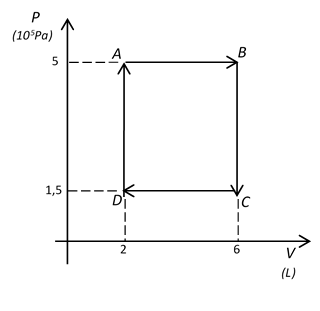
\includegraphics{./capitulo_04/termodin.png}
\caption{Ejemplificación de diagrama en blanco y negro.}
\label{fig:termodin}
\end{center}
\end{figure}

Las tablas deberían contener datos representativos que sinteticen información significativa del trabajo, evitando mostrar datos intermedios que pudieran dificultar la interpretación del mismo.

Cada tabla debe estar antecedida de un epígrafe que la identifique, enumere y describa brevemente.

Cada tabla debe ser referenciada al menos una vez, a través de su número, de preferencia antes de que aparezca en el documento, como en este caso (tabla \ref{tab:animales}).

\begin{table}[H]
\begin{center}
\caption{Inventario de animales.}
\label{tab:animales}
\begin{tabular}{||l|l|r||}
\hline
Especie&Sexo&Cantidad\\
\hline
\multirow{2}{*}{palomas}&jóvenes&20\\
&adultas&18\\
\hline
\multirow{2}{*}{conejos}&jóvenes&5\\
&adultos&5\\
\hline
\multirow{2}{*}{gallinas}&jóvenes&50\\
&adultas&50\\
\hline
\multicolumn{2}{||c|}{Total}&148\\
\hline
\end{tabular}
\end{center}
\end{table}

Otro ejemplo de tabla en el cual se observa el empleo de color, además de la combinación de columnas se observa en la tabla \ref{tab:color}

\begin{table}[H]
\begin{center}
\caption{Clasificación de la muestra, por edad.}
\label{tab:color}
\begin{tabular}{|c|cccc|}
\hline
\multirow{2}{*}{\cellcolor[rgb]{0.4,0.8,0.5}} &  \multicolumn{4}{>{\cellcolor[rgb]{0.4,0.8,0.9}}c|}{Tamaño de las muestras} \\ 
\cellcolor[rgb]{0.4,0.8,0.5}Edad&\cellcolor[rgb]{0.4,0.8,0.9} San Lorenzo &\cellcolor[rgb]{0.4,0.8,0.9} Asunción &\cellcolor[rgb]{0.4,0.8,0.9} Villarrica &\cellcolor[rgb]{0.4,0.8,0.9} Encarnación \\
\hline
e$<$20 &  93 &  74 &  68 & 87 \\
19$<$e$<$40 &  52 &  48 &  69 & 70 \\
39$<$e$<$60 &  47 &  85 &  81 & 64 \\
59$<$e$<$80 &  28 &  36 &  16 & 23 \\
79$<$e &  9 &  5 &  6 & 12 \\
\hline 
\end{tabular}
\end{center}
\end{table}

Aveces, como en el caso de la tabla \ref{tab:color}, el código se vuelve bastante complejo que resulta engorroso obtener en tiempo razonable la apariencia esperada de la tabla. En esos casos; es posible elaborar la tabla en entorno diferente a Latex; grabarla como imagen png, o jpg, o pdf; e insertarla enmascarada como tabla para ser contada como una de ellas por el contador de tablas: esto se logra con incluir la imagen dentro del entorno ``table'', como se ejemplifica con la tabla \ref{tab:tabla_word} que sigue.

\begin{table}[H]
	\begin{center}
		\caption{Imagen de tabla, en reemplazo de la tabla anterior.}
		\label{tab:tabla_word}
		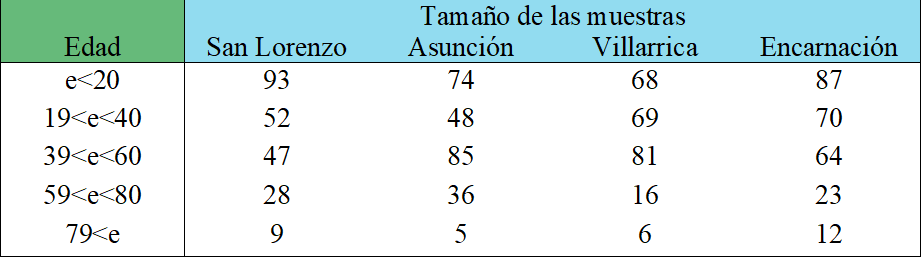
\includegraphics[scale=.65]{./capitulo_04/tabla_word.png}
	\end{center}
\end{table}


\fancyhead{}
\fancyfoot{}
\cfoot{\thepage}

\lhead{Discusión}

\chapter{Discusión}

El desarrollo del sistema automatizado de control de asistencia mediante reconocimiento facial en la FPUNE permitió abordar una problemática concreta y recurrente en los entornos académicos: la gestión precisa, ágil y confiable de la asistencia estudiantil. A lo largo de esta investigación, se cumplieron los objetivos propuestos y se obtuvo una solución funcional basada en tecnologías de visión artificial.

Los resultados experimentales obtenidos muestran que, con una configuración adecuada de los parámetros del sistema —como el umbral de similitud y el modelo de reconocimiento—, es posible lograr un desempeño óptimo tanto en precisión como en velocidad de procesamiento. Por ejemplo, al aplicar configuraciones con umbrales entre 1.0 y 1.8 y ajustar el factor de similitud, se observó un control eficaz sobre los falsos positivos, lo cual refuerza la aplicabilidad del sistema en entornos reales. Estos hallazgos coinciden con estudios previos en los que se destaca la sensibilidad de los sistemas biométricos ante condiciones de iluminación, ángulo y calidad de imagen.

Asimismo, se comprobó que modelos como YOLOv8n-Face y ArcFace ofrecen un equilibrio ideal entre precisión, rendimiento y tamaño del modelo, lo que los convierte en opciones viables para instituciones con recursos limitados. Este punto representa un avance sobre propuestas anteriores que requerían hardware especializado o mantenían altas tasas de error.


Entre las limitaciones encontradas, se destaca la sensibilidad a las condiciones de captura (especialmente iluminación y expresión), así como la necesidad de contar con múltiples imágenes por usuario para reducir el margen de error. Estas cuestiones abren la puerta a futuras investigaciones que busquen mejorar la robustez del sistema, integrar técnicas de aprendizaje continuo o ampliar la base de datos con más diversidad.

Finalmente, la experiencia de implementación dejó en evidencia que la automatización del control de asistencia no solo es técnicamente posible, sino también beneficiosa desde el punto de vista administrativo, al reducir errores humanos y optimizar los procesos de control en clase. En este sentido, el sistema desarrollado no solo respondió a las preguntas de investigación, sino que aportó evidencia concreta para su posible adopción e implementación institucional.


\section{Logros alcanzados}

El proyecto logró implementar un sistema funcional de asistencia basado en reconocimiento facial adaptado a las condiciones técnicas y operativas de la FPUNE. A lo largo del desarrollo se cumplieron los objetivos específicos planteados: se evaluaron diferentes modelos de reconocimiento facial, se seleccionaron las tecnologías más adecuadas (YOLOv8 y ArcFace), y se diseñó un flujo completo de captura, detección, extracción de características y verificación.

Además, se realizaron pruebas en distintas condiciones de iluminación, ángulo y expresión facial, lo que permitió validar la efectividad del sistema frente a escenarios reales. Las configuraciones óptimas (por ejemplo, con umbrales de distancia entre 1.3 y 1.8) demostraron un buen equilibrio entre precisión y tolerancia a variaciones.

El sistema también fue evaluado en tiempo de ejecución y mostró buen rendimiento en hardware accesible, lo que valida su aplicabilidad en entornos académicos con recursos limitados. Se documentaron los ajustes aplicados para mejorar la precisión y reducir falsos positivos, destacando la importancia del preprocesamiento, la segmentación por identidad y el uso de índices embebidos en memoria.

\section{Solución del problema de investigación}

El problema identificado fue la necesidad de automatizar el registro de asistencia de alumnos en la FPUNE utilizando tecnologías confiables y no intrusivas. A través del enfoque aplicado, se logró resolverlo con un sistema que captura rostros en tiempo real, identifica a los estudiantes registrados y registra automáticamente su presencia, eliminando procesos manuales.

Los resultados obtenidos permiten afirmar que el sistema desarrollado cumple con su propósito principal: registrar de forma precisa, rápida y automática la asistencia de los estudiantes.

Además, se logró responder adecuadamente a las preguntas de investigación planteadas y se comprobó la hipótesis inicial. Esto valida tanto la viabilidad técnica como la operatividad del sistema en el contexto académico local, demostrando su aplicabilidad en entornos reales.

\section{Sugerencias para futuras investigaciones}

{\renewcommand{\labelitemi}{\textbullet}
\begin{itemize}
    \item \textbf{Integrar verificación por doble factor} (como código QR, tarjetas inteligentes o tecnología NFC) para reforzar los mecanismos de autenticación en situaciones críticas. Esta medida podría ser especialmente útil en exámenes, actividades de alta importancia académica o en contextos donde se requiera una mayor seguridad en la verificación de identidad.
    
    \item \textbf{Evaluar el desempeño del sistema con una base de datos más amplia y heterogénea}, que incorpore mayor cantidad de estudiantes, con variaciones demográficas como edad, género, etnia y condiciones lumínicas diversas. Esto permitiría validar la robustez del modelo en un entorno más realista y adaptable.
    
    \item \textbf{Adaptar el sistema a dispositivos móviles o cámaras IP} con transmisión remota para su uso en aulas híbridas o espacios no convencionales. Esta implementación favorecería la escalabilidad del sistema, permitiendo su uso más allá de los laboratorios o aulas tradicionales, incluso en entornos con conexión limitada o uso descentralizado.
    
    \item \textbf{Aplicar técnicas de aprendizaje continuo o incremental}, de forma que el modelo de reconocimiento facial pueda actualizarse progresivamente a partir de nuevas muestras capturadas, sin necesidad de un reentrenamiento completo. Esta característica no solo mejora la precisión con el tiempo, sino que además optimiza los recursos computacionales y mantiene el sistema actualizado con los cambios faciales naturales de los estudiantes (como uso de anteojos, barba, etc.).
    
    \item \textbf{Explorar el uso de técnicas de anonimización o protección de datos biométricos}, cumpliendo con principios de privacidad y legislación vigente (como la Ley de Protección de Datos Personales), de modo que el sistema pueda escalar institucionalmente sin comprometer la seguridad de la información.
\end{itemize}


\backmatter

\cleardoublepage
\addcontentsline{toc}{chapter}{Glosario}
\printglossary
% \printglossaries

\addcontentsline{toc}{chapter}{Anexos}

\cleardoublepage
\fancyhead{}
\fancyfoot{}
\cfoot{\thepage}

\lhead{Anexo A.}
%\rhead{\today}
%\rfoot{\thepage}

\chapter{Anexo A.}
Los apéndices y anexos resultan útiles para describir con mayor profundidad ciertos materiales, sin distraer la lectura del texto principal del reporte o evitar que rompan con el formato de éste. Algunos ejemplos serían el cuestionario utilizado, un código de programa computacional, análisis estadísticos adicionales, la demostración matemática de un teorema complicado, fotografías testimoniales, etc.



\cleardoublepage
\addcontentsline{toc}{chapter}{Referencias bibliogr\'aficas}

\bibliographystyle{IEEEtran-castellano}
\bibliography{test}

\end{document}

